%% LyX 2.0.0rc3 created this file.  For more info, see http://www.lyx.org/.
%% Do not edit unless you really know what you are doing.
\documentclass[english]{beamer}
\usepackage{mathptmx}
\renewcommand{\familydefault}{\rmdefault}
\usepackage[T1]{fontenc}
\usepackage[latin9]{inputenc}
\usepackage{color}
\usepackage{textcomp}
\usepackage{amsmath}
\usepackage{amssymb}
\usepackage{graphicx}

\makeatletter

%%%%%%%%%%%%%%%%%%%%%%%%%%%%%% LyX specific LaTeX commands.
\newcommand{\lyxmathsym}[1]{\ifmmode\begingroup\def\b@ld{bold}
  \text{\ifx\math@version\b@ld\bfseries\fi#1}\endgroup\else#1\fi}

%% Because html converters don't know tabularnewline
\providecommand{\tabularnewline}{\\}

%%%%%%%%%%%%%%%%%%%%%%%%%%%%%% Textclass specific LaTeX commands.
 % this default might be overridden by plain title style
 \newcommand\makebeamertitle{\frame{\maketitle}}%
 \AtBeginDocument{
   \let\origtableofcontents=\tableofcontents
   \def\tableofcontents{\@ifnextchar[{\origtableofcontents}{\gobbletableofcontents}}
   \def\gobbletableofcontents#1{\origtableofcontents}
 }
 \long\def\lyxframe#1{\@lyxframe#1\@lyxframestop}%
 \def\@lyxframe{\@ifnextchar<{\@@lyxframe}{\@@lyxframe<*>}}%
 \def\@@lyxframe<#1>{\@ifnextchar[{\@@@lyxframe<#1>}{\@@@lyxframe<#1>[]}}
 \def\@@@lyxframe<#1>[{\@ifnextchar<{\@@@@@lyxframe<#1>[}{\@@@@lyxframe<#1>[<*>][}}
 \def\@@@@@lyxframe<#1>[#2]{\@ifnextchar[{\@@@@lyxframe<#1>[#2]}{\@@@@lyxframe<#1>[#2][]}}
 \long\def\@@@@lyxframe<#1>[#2][#3]#4\@lyxframestop#5\lyxframeend{%
   \frame<#1>[#2][#3]{\frametitle{#4}#5}}
 \def\lyxframeend{} % In case there is a superfluous frame end

%%%%%%%%%%%%%%%%%%%%%%%%%%%%%% User specified LaTeX commands.
\usepackage{amsfonts}

\usetheme{Madrid}

%\usetheme{Warsaw}
% or ...

%\setbeamercovered{transparent}
% or whatever (possibly just delete it)

\newcounter{esr}
\newtheorem{esercizio}[esr]{Exercise}

\makeatother

\usepackage{babel}
\begin{document}

\title{Statistics Lecture}


\author{Claudio Ortelli~\inst{1}}


\institute{\inst{1} Finance Institute\\
Universit� della Svizzera italiana}


\date[ALARI 2011]{Advanced Learning and Research Institute, 2011}

\makebeamertitle
\section{Continuous random variables}

\subsection{Exponential distribution}

 \begin{frame}{Continuous random variables}{Exponential distribution}
The exponential distribution find its application in reliability theory
and queuing theory. The following random variables are often modeled
as exponential: 
\begin{enumerate}
\item Time between two successive job arrivals to a file server (often called \textbf{interarrival time}). 
\item Service time at a server in a queuing network; the server could be
a resource such as a CPU, an I/O device, or a communication channel.
\item Time to failure (lifetime) of a component. 
\item Time required to repair a component that has malfunctioned. 
\end{enumerate}
\textbf{Remark:} The choice of the exponential distribution to model
the stochastic structure of the upper described variables is an assumption
and not a given fact! Experimental verification of the distributional
assumption will be therefore necessary before to relying on the results
of the analysis. 

\end{frame}

\begin{frame}{Continuous random variables}{The memoryless property
of the exponential distribution} Le $X\sim Exp(\lambda)$ be the
lifetime of a component. Suppose we have observed that it has already
been operating for $t$ hours. 
\begin{itemize}
\item What is the distribution of the remaining (residual) lifetime $Y=X-t$? 
\end{itemize}
Let the conditional probability of $Y\leq y$, given that $X>t$,
be denoted by $G_{Y}(y\rvert t)$. For $y\geq0$

\begin{eqnarray*}
G_{Y}(y\rvert t) & = & P(Y\leq y\rvert X>t)=\frac{P(\{Y\leq y\}\textnormal{ and }\{X>t\})}{P(X>t)}\\
 & = & \frac{P(\{X\leq y+t\}\textnormal{ and }\{X>t\})}{P(X>t)}=\frac{P(t<X\leq y+t)}{P(X>t)}\\
 & = & \frac{exp(-\lambda t)(1-exp(-\lambda y))}{exp(-\lambda t)}=1-exp(-\lambda y).
\end{eqnarray*}
 \end{frame}

\begin{frame}{Continuous random variables}{The memoryless property
of the exponential distribution} \textbf{Result:}\\
 The conditional distribution $G_{Y}(y\rvert t)$ does not depend
on $t$ and is identical to the distribution of $X$, i.e. $Exp(\lambda)$.\\
 \vspace{1cm}
 \textbf{Interpretation:}\\
 The distribution of the remaining life does not depend on how long
the component has been operating, i.e. the component does not age
(it is as good as new). Therefore, the exponential distribution is
not suited to model components or devices that gradually deteriorate.

\end{frame}

\subsection{Reliability and failure rate}

\begin{frame}{Continuous random variables}{The reliability and
failure rate} Let the random variable $X$ be the lifetime (or time
to failure) of a component. \begin{definition} The \textbf{reliability}
$R(t)$ of the component is the probability that the component survives
until some time $t$, i.e. 
\[
R(t)=P(X>t)=1-F_{X}(t)
\]
 $F_{X}(t)$ is often called the \textbf{unreliability} of the component.
\end{definition} The conditional probability that the component \textcolor{red}{does
not} survive for an additional interval of duration $x$ given that
it has survived until time $t$ is equal to 
\[
G_{Y}(x\rvert t)=\frac{P(t<X\leq t+x)}{P(X>t)}=\frac{F_{X}(t+x)-F_{X}(t)}{R(t)}
\]
 \end{frame}

\begin{frame}{Continuous random variables}{The reliability and
failure rate} \begin{definition} The instantaneous failure rate
$h(t)$ is defined to be 
\[
h(t)=\lim_{x\rightarrow0}\frac{1}{x}G_{Y}(x\rvert t)=\lim_{x\rightarrow0}\frac{F_{X}(t+x)-F_{X}(t)}{xR(t)}\ ,
\]
 so that 
\[
h(t)=\frac{f_{X}(t)}{R(t)}.
\]
 \end{definition} Alternate terms for $h(t)$ are \textit{hazard
rate}, \textit{force of mortality}, \textit{intensity rate}, \textit{conditional
failure rate} or \textbf{failure rate}.\\
 Interpretation: 
\begin{itemize}
\item $h(t)\Delta t$ represents the conditional probability that a component
having survived to age $t$ will fail in the interval $(t,t+\Delta t]$. 
\end{itemize}
\end{frame}

\begin{frame}{Continuous random variables}{The reliability and
failure rate}%[allowframebreaks]

\begin{itemize}
\item $f_{X}(t)\Delta t$ is the \textit{unconditional} probability while
$h(t)\Delta t$ is a conditional probability. 
\end{itemize}
Next theorem shows the connection between reliability and failure
rate. \begin{theorem} 
\[
R(t)=\exp\left(-\int_{0}^{t}h(x)dx\right)
\]
 \end{theorem} \begin{proof} 
\[
\int_{0}^{t}h(x)dx=\int_{0}^{t}\frac{f_{X}(x)}{R(x)}dx=\int_{0}^{t}\frac{-R'(x)}{R(x)}dx=-\ln(R(t))
\]
 using the fact that $R'(x)=-f_{X}(x)$ and the boundary contition
$R(0)=1$. \end{proof}

\end{frame}

\begin{frame}{Continuous random variables}{The reliability and
failure rate} \begin{definition} The cumulative hazard is defined
to be 
\[
H(t)=\int_{0}^{t}h(x)dx
\]
 \end{definition} Then, reliability can also be written as $R(t)=\exp(-H(t))$.
\begin{definition}\label{DefConditionalReliability} The conditional
reliability $R_{t}(y)$ is the probability that the component survives
an additional interval of duration $y$ given that it has survived
until time $t$. 
\begin{eqnarray}
R_{t}(y)=\frac{R(t+y)}{R(t)}\label{conditionalReliability}
\end{eqnarray}
\end{definition} \end{frame}

\begin{frame}{Continuous random variables}{The reliability and
failure rate} Assume a component does not age stochastically, i.e.
the survival probability over an additional time interval $y$ is
the same regardless of the age $t$ of the component: 
\begin{eqnarray*}
R_{t}(y) & = & R_{s}(y)\textnormal{ \ for all }t,s\geq0.
\end{eqnarray*}
Thus, for $s=0$ 
\begin{eqnarray*}
R_{t}(y) & = & R_{0}(y)=\frac{R(y)}{R(0)}=R(y),
\end{eqnarray*}
 so that from $R_{t}(y)=R(t+y)/R(t)$ we have 
\begin{eqnarray*}
R(t+y) & = & R(t)R(y).
\end{eqnarray*}
 In particular we obtain 
\begin{eqnarray*}
\frac{R(t+y)-R(y)}{t} & = & \frac{(R(t)-1)R(y)}{t}=\frac{(R(t)-R(0))R(y)}{t}.
\end{eqnarray*}
 \end{frame}

\begin{frame}{Continuous random variables}{The reliability and
failure rate} Taking the limit as $t\rightarrow0$ 
\begin{eqnarray*}
R'(y) & = & R'(0)R(y)\\
R(y) & = & \exp(yR'(0))=\exp(-\lambda y)
\end{eqnarray*}
 which shows that the lifetime $X\sim Exp(\lambda)$.\\
 If a component has exponential lifetime distribution it follows that 
\begin{enumerate}
\item A replacement policy of used components based on the lifetime of the
components is useless. 
\item In estimating mean life and reliability the age of the observed components
are of no concern. The number of hours of observed live and the number
of observed failures are of interest. 
\end{enumerate}
\end{frame}

\begin{frame}{Continuous random variables}{The reliability and
failure rate} \begin{definition} Increasing (decreasing) failure
rate distribution\\
 Let $X$ be the lifetime of a component and $F_{X}(t)$ the corresponding
distribution function. If its failure rate $h(t)$ is an increasing
(decreasing) function of $t$ for $t\geq0$ then $F_{X}$ is an Increasing
(Decreasing) Failure Rate distribution: IFR (DFR) distribution. \end{definition}

\end{frame} \begin{frame}{Continuous random variables}{The reliability
and failure rate} The behavior of the failure rate $h(t)$ as a function
of age is known as the \textit{mortality curve}, \textit{hazard function},
\textit{life characteristic} or \textit{lambda characteristic}. 

\begin{center}
\includegraphics[width=110pt,keepaspectratio]{Figura3_6} % Figura3.6: 336x256 pixel, 90dpi, 9.48x7.23 cm, bb=0 0 269 205

\par\end{center}

\end{frame}

\begin{frame}{Continuous random variables}{The reliability and
failure rate}

\begin{esercizio}
\begin{enumerate}
\item The failure rate of a certain component is $h(t)=\lambda_{0}t$, where
$\lambda_{0}>0$ is a given constant. Determine the reliability, $R(t)$,
of the component. Repeat for $h(t)=\lambda_{0}t^{1/2}$.
\item The failure rate of a computer system for onboard control of a space
vehicle is estimated to be the following function of time:
\[
h(t)=\alpha\mu t^{\alpha-1}+\beta\gamma t^{\beta-1}.
\]
Derive an expression for the reliability $R(t)$ of the system. Plot
$h(t)$ and $R(t)$ as functions of time with parameter values $\alpha=\frac{1}{4}$,
$\beta=\frac{1}{7}$, $\mu=0.0004$ and $\gamma=0.0007$.
\end{enumerate}
\end{esercizio}

\end{frame}

\subsection{Important distributions}

\subsubsection{Hypoexponential Distribution}

\begin{frame}{Continuous random variables}{Hypoexponential Distribution}
The hypoexponential distribution is used to model processes that can
be divided into sequential phases such that the time the process spends
in each phase is independent and exponentially distributed. 
\begin{itemize}
\item Service times for input-output operations in a computer system often
follow this distribution. 
\end{itemize}
A two stage hypoexponential random variable $X\sim Hypo(\lambda_{1},\lambda_{2})$
has pdf and distribution function equal to 
\begin{eqnarray*}
f(t) & = & \frac{\lambda_{1}\lambda_{2}}{\lambda_{2}-\lambda_{1}}(\exp(-\lambda_{1}t)-\exp(\lambda_{2}t)),\ \ t>0\\
F(t) & = & 1-\frac{\lambda_{2}}{\lambda_{2}-\lambda_{1}}\exp(-\lambda_{1}t)+\frac{\lambda_{1}}{\lambda_{2}-\lambda_{1}}\exp(-\lambda_{2}t)
\end{eqnarray*}


\end{frame}

\subsubsection{Erlang Distribution}

\begin{frame}{Continuous random variables}{Erlang Distribution}
When $r$ sequential phases have identical exponential distribution
the resulting density is known as $r-$stage Erlang and is given by

\begin{eqnarray*}
f(t) & = & \frac{\lambda^{r}t^{r-1}\exp(-\lambda t)}{(r-1)!}\textnormal{ with }t>0,\ \lambda>0,\ r=1,2,\dots\\
F(t) & = & 1-\sum_{k=0}^{r-1}\frac{(\lambda t)^{k}}{k!}\exp(-\lambda t)\textnormal{ with }t\geq0,\ \lambda>0,\ r=1,2,\dots
\end{eqnarray*}


\end{frame}

\subsubsection{Hyperexponential Distribution}

\begin{frame}{Continuous random variables}{Hyperexponential Distribution}
Suppose that a process consists of alternate phases, i.e. during any
single experiment the process experiences one and only one of the
many alternate phases, and these phases have exponential distributions.
The overall distribution is then hyperexponential with density and
distribution functions given by

\begin{eqnarray*}
f(t) & = & \sum_{i=1}^{k}\alpha_{i}\lambda_{i}\exp(-\lambda_{i}t)\textnormal{ with }t>0,\ \lambda_{i}>0,\ \sum_{i=1}^{k}\alpha_{i}=1\\
F(t) & = & \sum_{i}\alpha_{i}(1-\exp(\lambda_{i}t))\ \ t\geq0
\end{eqnarray*}


\end{frame}

\subsubsection{Weibull Distribution}

\begin{frame}{Continuous random variables}{Weibull Distribution}
The Weibull distribution is the most widely used parametric family
of failure distributions. It has been used to describe 
\begin{itemize}
\item fatigue failure 
\item electronic component failure 
\item ballbearing failure 
\end{itemize}
The reason is that by a proper choice of the shape parameter $\alpha$
we can obtain an IFR, DFR or constant failure rate distribution. The
corresponding density and distribution functions are given by

\begin{eqnarray*}
f(t) & = & \lambda\alpha t^{\alpha-1}\exp(-\lambda t^{\alpha})\\
F(t) & = & 1-\exp(-\lambda t^{\alpha})
\end{eqnarray*}
 where $t\geq0$, $\lambda>0$ and $\alpha>0$. \end{frame}

\subsubsection{Pareto Distribution}

\begin{frame}{Continuous random variables}{Pareto Distribution}
The Pareto (also knonw as double-exponential, hyperbolic or power-law)
distribution has been used to model 
\begin{itemize}
\item the amount of CPU time consumed by an arbitrary process 
\item the Web file size on the Internet servers 
\item the thinking time of the web browser 
\item the number of data bytes in FTP bursts 
\item the access frequency of Web traffic 
\end{itemize}
The density and distributions functions are given by 
\begin{eqnarray*}
f(x) & = & \alpha k^{\alpha}x^{-\alpha-1}\ \ x\geq k,\ k>0,\ \alpha>0\\
F(x) & = & \left\{ \begin{array}{ll}
1-\left(\frac{k}{x}\right)^{\alpha} & \ x\geq k\\
0 & x<k
\end{array}\right.
\end{eqnarray*}
 \end{frame}

\begin{frame}{Continuous random variables}

\begin{esercizio}
\begin{enumerate}
\item Show that the failure rate $h(t)$ of the hypoexponential distribution
has the property 
\[
\underset{t\rightarrow+\infty}{lim}h(t)=min\{\lambda_{1},\lambda_{2}\}.
\]

\item Show that a two-stage Erlang pdf is the limiting case of two-stage
hypoexponential pdf. In other words, show that 
\[
\underset{t\rightarrow+\infty}{lim}\frac{\lambda_{1}\lambda_{2}}{\lambda_{2}-\lambda_{1}}(e^{-\lambda_{1}t}-e^{-\lambda_{2}t})=\lambda_{2}^{2}te^{-\lambda_{2}t}.
\]
(Hint: Use l'H�pital's rule.)
\item The CPU time requirement of a typical program measured in minutes
is found to follow a three-stage Erlang distribution with $\lambda=0.5$.
What is the probability that the CPU demand of a program will exceed
1 minute?
\end{enumerate}
\end{esercizio}

\end{frame}

\section{Functions of random variables}


\lyxframeend{}\lyxframe{Functions of random variables}
\begin{itemize}
\item Let $X$ be a continuous random variable with distribution function
$F_{X}$, $\Psi$ a function and 
\[
Y=\Psi(X).
\]

\item Under regularity conditions on $\Psi$, $Y$ is a random variable! 
\item Continuity or stepwise continuity of $\Psi$ are sufficient conditions
for $Y$ to be a random variable. \end{itemize}
\begin{exampleblock}
{Example: Quadratic cost function.} 

Let $X$ denote a measurement error. We assume a quadratic cost function,
i.e. $Y=\Psi(X)=X^{2}$. The random variable $Y$ has a distribution
function $F_{Y}$ which depends on $F_{X}$ and $\Psi$.
\end{exampleblock}

\lyxframeend{}


\lyxframeend{}\lyxframe{Functions of random variables}
\begin{itemize}
\item To derive $F_{Y}$ simply compute the preimage of the event $C=(-\infty,y]$.
In fact by definition of $F_{Y}$
\begin{eqnarray*}
F_{Y}(y) & = & P(Y\leq y)=P(Y\in C)\\
 & = & P(\Psi(X)\in C)\\
 & = & P(\Psi^{-1}(C))\\
 & = & P_{X}(B)
\end{eqnarray*}
where the set $B$ is the preimage of $C$, i.e.
\[
B=\Psi^{-1}(C)=\{x\in\mathbb{R\mid}\Psi(x)\in C\}.
\]

\item The preimage function of $\Psi$ is a set function (the arguments
are subsets of $\mathbb{R}$) and is defined even if $\Psi$ is not
one-to-one.
\end{itemize}

\lyxframeend{}


\lyxframeend{}\lyxframe{Functions of random variables}

\noindent \begin{center}
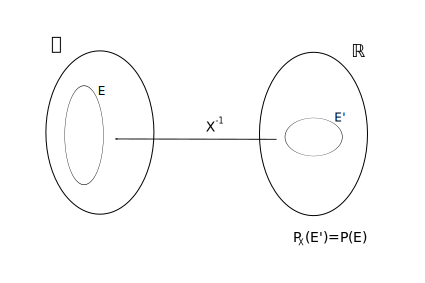
\includegraphics{codiceR/grafici/variabileAleatoria}
\par\end{center}


\lyxframeend{}\lyxframe{Functions of random variables}

\noindent \begin{center}
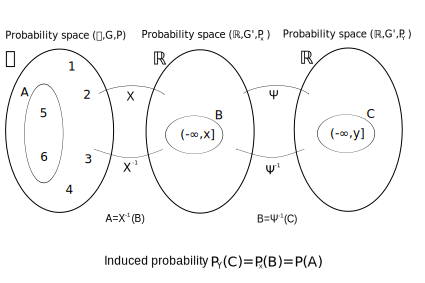
\includegraphics[scale=0.95]{codiceR/grafici/funzioneDivariabileAleatoria}
\par\end{center}


\lyxframeend{}\lyxframe{Functions of random variables}
\begin{exampleblock}
{Example continued}

Because $Y=X^{2}$ is always positive $F_{Y}(y)=0$ whenever $y\leq0$.
When $y>0$ it follows $Y\leqslant y\Leftrightarrow-\sqrt{y}\leqslant X\leqslant\sqrt{y}$
so that $F_{Y}(y)=F_{X}(\sqrt{y})-F_{X}(-\sqrt{y})$. If the random
variable $X$ has a density function we can differentiate the last
expression to obtain the density function of $Y$:
\[
f_{Y}(y)=\begin{cases}
\frac{1}{2\sqrt{y}}\left[f_{X}(\sqrt{y})+f_{X}(-\sqrt{y})\right], & y>0,\\
0, & \mbox{otherwise.}
\end{cases}
\]

\end{exampleblock}
\begin{esercizio}Let $X$ be uniformly distributed on $(0,1)$ and
define $Y=-\lambda^{-1}ln(1-X)$ where $\lambda>0$ is a parameter.
Show that $Y$ has an exponential distribution with parameter $\lambda$. 

\end{esercizio}


\lyxframeend{}


\lyxframeend{}\lyxframe{Functions of random variables}
\begin{theorem}%{}
\label{the:transform theorem}Let $X$ be a continuous random variable
with density function $f_{X}$ satisfying 
\begin{itemize}
\item $f_{X}>0$ for $x\in I\subset\mathbb{R}$ and 
\item $f_{X}>0$ for $x\notin I$ 
\end{itemize}
and let $\Phi$ be a \emph{differentiable} and \emph{monotone} real
valued function with domain $I$. Then $Y=\Phi(X)$ is a continuous
random variable with density function
\[
f_{Y}(y)=\begin{cases}
f_{X}\left[\Phi^{-1}(y)\right]\left[\mid\frac{\partial}{\partial y}\left(\Phi^{-1}\right)(y)\mid\right], & y\in\Phi(I),\\
0, & \mbox{otherwise.}
\end{cases}
\]

\end{theorem}%{}

\lyxframeend{}


\lyxframeend{}\lyxframe{Functions of random variables}
\begin{examples}%{}
1) Let $\Phi$ be the distribution function $F$ of the random variable
$X$ with density function $f$ (we need to assume that $F$ has the
previous properties of continuity and differentiability) and define
$Y=F(X)$. The random variable $Y$ has density given by 
\[
f_{Y}(y)=\begin{cases}
1, & 0<y<1,\\
0, & \mbox{otherwise}.
\end{cases}
\]


2) Assume $Y=aX+b$, i.e. $Y$ is a affine linear trasformation of
$X$. By the previous Theorem we have that ($I$ is the set over which
$f_{X}\neq0$) 
\[
f_{Y}(y)=\begin{cases}
\frac{1}{\mid a\mid}f_{X}\left(\frac{y-b}{a}\right), & y\in aI+b,\\
0, & \mbox{otherwise.}
\end{cases}
\]



\end{examples}%{}

\lyxframeend{}


\lyxframeend{}\lyxframe{Functions of random variables}

\begin{esercizio}
\begin{enumerate}
\item In the second part of the previous Example assume that $X\thicksim N(\mu,sigma^{2})$
and derive the density function of $Y$. What do you observe?
\item Let as before $X$ be $N(\mu,sigma^{2})$ and assume $Y=e^{X}$. Derive
the density and distribution function of $Y$.
\item Show that if $X$ has the $k-$stage Erlang distribution with parameter
$\lambda$, then $Y=2\lambda X$ has the $chi-$square distribution
with $2k$ degrees of freedom.
\end{enumerate}
\end{esercizio}


\lyxframeend{}

\section{Jointly distributed random variables}

\begin{frame}{Jointly distributed random variables}

\includegraphics[scale=0.35]{/home/claudio/eclipse/grafici-stat2/alari/jointlyDistributedRandomVariables}

\end{frame}

\begin{frame}{Jointly distributed random variables}

\includegraphics[scale=0.35]{/home/claudio/eclipse/grafici-stat2/alari/jointlyDistributedRandomVariables1}

\end{frame}

\begin{frame}{Jointly distributed random variables}

\includegraphics[scale=0.35]{/home/claudio/eclipse/grafici-stat2/alari/jointlyDistributedRandomVariables2}

\end{frame}

\begin{frame}{Jointly distributed random variables}

\includegraphics[scale=0.35]{/home/claudio/eclipse/grafici-stat2/alari/jointlyDistributedRandomVariables3}

\end{frame}

\section{Simulation of random variables}

\begin{frame}{Simulation of random variables}{Motivation} 
\begin{itemize}
\item We are interested in simulating a model of a real system (network,
electronic device, ...). 
\item The output $Y$ of the model depends on a stochastic input, i.e. a
random variable $X$ with known distribution function $F_{X}$: 
\[
Y=g(X).
\]
 
\end{itemize}
\begin{center}
\includegraphics[width=157pt,keepaspectratio]{sistemaComplesso} % sistemaComplesso.png: 314x158 pixel, 72dpi, 11.08x5.57 cm, bb=0 0 314 158

\par\end{center}

\end{frame}


\lyxframeend{}\lyxframe{Simulation of random variables}
\begin{itemize}
\item The model is too complex in order to analytically derive the probabilistic
properties of the output, i.e. $F_{Y}$. 
\item Idea: simulate a possible outcome $x$ of the input $X$ and evaluate
the corresponding outcome $y=g(x)$ of the output. Repeat the experiment
$N$ times and analyse the results. 
\item The simulated values of the input must be drawn from the distribution
of $X$. 
\item Question: how is it possible to simulate independent realizations
from a given distribution $F_{X}$? 
\item Answer: different methods available. The simplest of them requires
simulating from the uniform distribution on the open interval (0,1),
i.e. $U(0,1)$. In Matlab use the function {}``rand''. 
\end{itemize}

\lyxframeend{}

\begin{frame}{Simulation of random variables}{Inverse Transform
Method} If the distribution function $F_{X}$ is continuous and strictly
increasing then $F_{X}^{-1}:\ (0,1)\rightarrow\mathbb{R}$ exists.
\\
 

\begin{center}
Example: Chi-Squared Distribution with 5 degrees of freedom 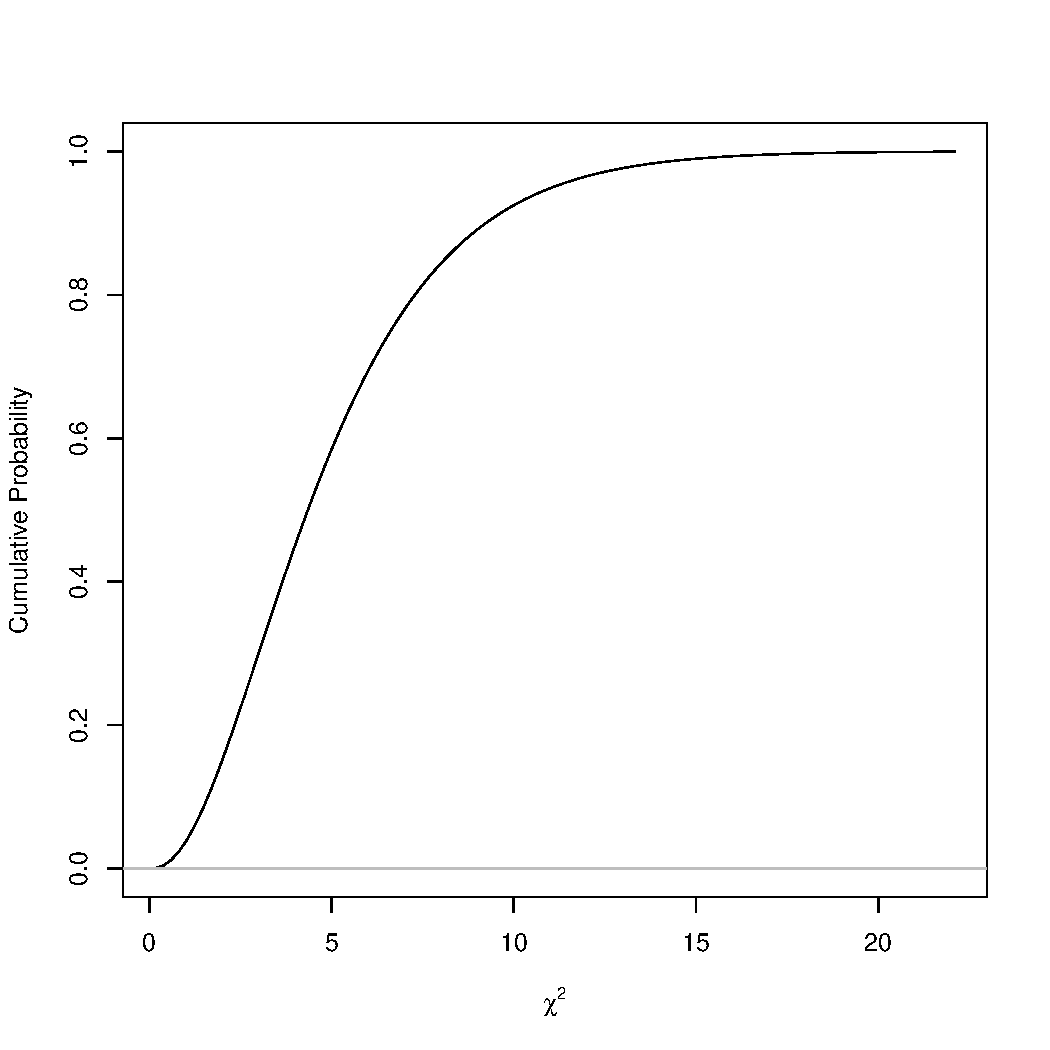
\includegraphics[width=5.8cm,keepaspectratio]{distChi2}
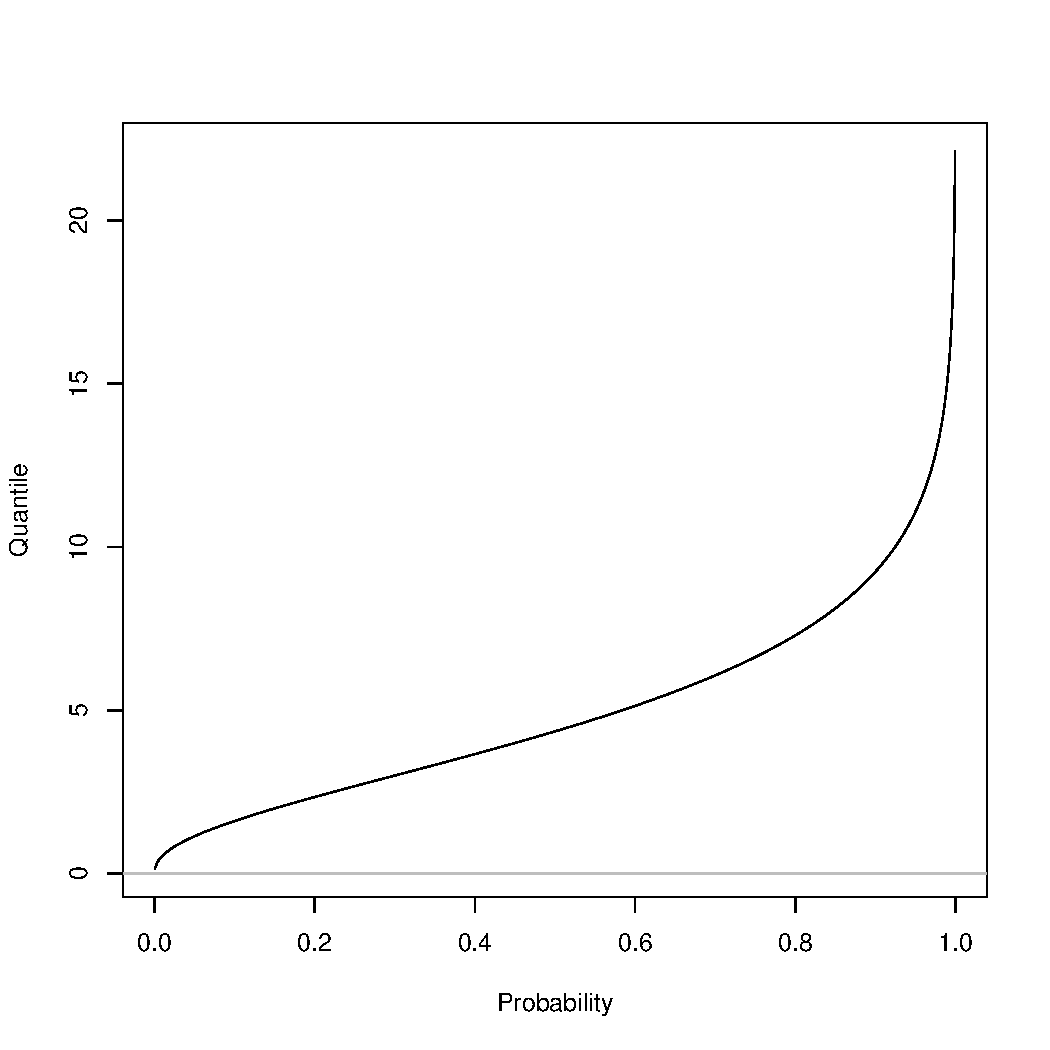
\includegraphics[width=5.8cm,keepaspectratio]{quantileChi2} 
\par\end{center}

\end{frame}

\begin{frame}{Simulation of random variables} For a general distribution
function not necessarily strictly increasing define 
\[
F_{X}^{-1}(p)=\inf\{x:p\leq F_{X}(x)\}\ \ 0<p<1.
\]
 It then follows that $F_{X}^{-1}(p)\leq x\Longleftrightarrow p\leq F_{X}(x).$
\vspace{0.2cm}
 

\begin{center}
Example: Binomial distribution $Bin(n=3,p=0.3)$ 
\par\end{center}

\vspace{-0.7cm}
 

\begin{center}
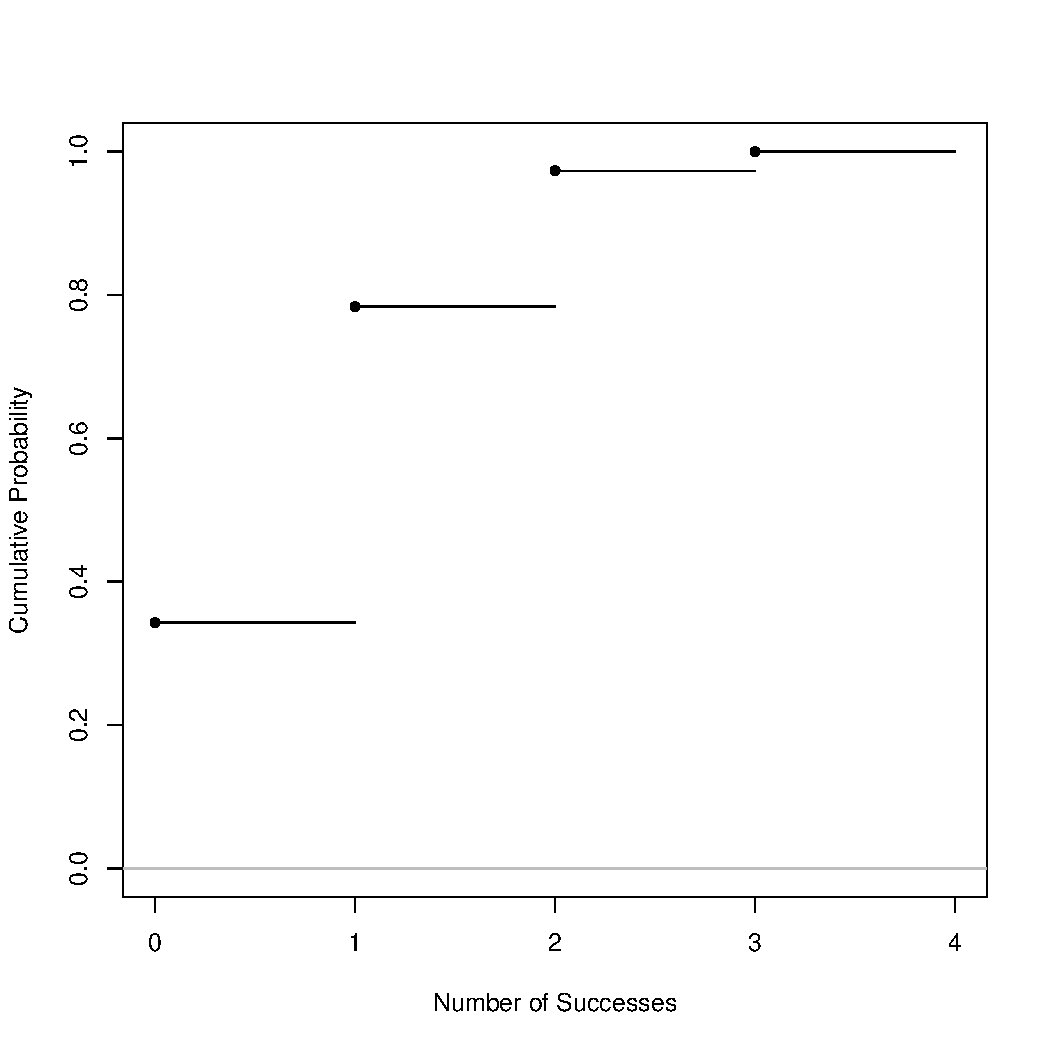
\includegraphics[width=5.8cm,keepaspectratio]{distBinomiale} \includegraphics[width=5.8cm,keepaspectratio]{quantileBinomiale} 
\par\end{center}

\end{frame}

\begin{frame}{Simulation of random variables}{Inverse Transform
Method} \begin{theorem}{[}Inverse Transform Method{]} Let $U$ a
continuous Unif(0,1) distributed random variable. The random variable
$Y=F_{X}^{-1}(U)$ has distribution function $F_{X}$. \end{theorem}
\begin{proof} By definition 
\[
F_{Y}(c):=P(Y\leq c)=P(F_{X}^{-1}(U)\leq c).
\]
 But the last equality is equivalent to (see previous slide) 
\[
P(U\leq F_{X}(c))=F_{X}(c).
\]
 \end{proof} \end{frame}

\begin{frame}{Simulation of random variables}{Inverse Transform
Method} From the previous theorem we derive the following \emph{two
steps} simulation algorithm 
\begin{enumerate}
\item Simulate a realization $u$ from a Unif(0,1) random variable $U$.
\item Compute $x=F_{X}^{-1}(u)$. \end{enumerate}
\begin{example}%{}
Simulation of $Y\sim Exp(\lambda)$
\begin{itemize}
\item The distribution function is $F_{Y}(x)=1-\exp(-\lambda x)$
\item Compute $F_{Y}^{-1}(p)=-\frac{1}{\lambda}\ln(1-p)$ 
\item Sample a random draw $u$ from $U\sim$ Unif(0,1)
\item Set $y=-\frac{1}{\lambda}\ln(1-u)$
\end{itemize}
\end{example}%{}
\end{frame}

\begin{frame}{Simulation of random variables}{Inverse Transform
Method} \vspace{-4cm}
 Remark: if $U\sim$ Unif(0,1) then $1-U$ is also Unif(0,1). Therefore
we can also write $Y=-\frac{1}{\lambda}\ln(U)$. \end{frame}

\begin{frame}{Simulation of random variables}{Inverse Transform
Method} For a descrete random variable $Y$ with probability mass
function $P(Y=x_{i})=p_{i}$, $i=1,...,m$ consider the following
algorithm: 
\begin{enumerate}
\item Generate a Unif(0,1) random variable $U$ 
\item Compute $Y$ as follows 
\[
Y=x_{j}\textnormal{\hspace{0.5cm} if \hspace{0.1cm}}\sum_{i=1}^{j-1}p_{i}<U\leq\sum_{i=1}^{j}p_{i}.
\]
 i.e. $Y=x_{j}$ if $F_{Y}(x_{j-1})<U\leq F_{Y}(x_{j})$. 
\end{enumerate}
\end{frame}

\begin{frame}{Simulation of random variables}{Inverse Transform
Method} 
\begin{example}%{}
Let $Y$ have the following mass function %
\begin{tabular}{|c|c|c|c|}
\hline 
$p_{1}$  & $p_{2}$  & $p_{3}$  & $p_{4}$\tabularnewline
\hline 
0.1  & 0.2  & 0.4  & 0.3 \tabularnewline
\hline 
\end{tabular}.

The simulation algorithm is the following:
\begin{enumerate}
\item If $u\leq p_{1}=0.1$ then $y=x_{1}$. Stop.
\item if $u\leq p_{1}+p_{2}=0.3$ then $y=x_{2}$. Stop. 
\item if $u\leq p_{1}+p_{2}+p_{3}=0.7$ then $y=x_{3}$. Stop. 
\item $y=x_{4}$. Stop. 
\end{enumerate}
This algorithm is correct but inefficient. In fact, probabilities
of one, two, ... comparisons are equal to the probabilities of $x_{1}$,
$x_{2}$, ..., respectively. The expected number of comparisons is
\[
p_{1}+2p_{2}+3p_{3}+4p_{4}=2.9.
\]

\end{example}%{}
\end{frame}

\begin{frame}{Simulation of random variables}{Inverse Transform
Method} We can improve efficiency by sorting the values of $x_{i}$
by decreasing order of probabilities $p_{i}$'s: $x_{3}$, $x_{4}$,
$x_{2}$ and $x_{1}$. 
\begin{enumerate}
\item If $u\leq p_{3}=0.4$ then $y=x_{3}$. Stop. 
\item if $u\leq p_{3}+p_{4}=0.7$ then $y=x_{4}$. Stop. 
\item if $u\leq p_{3}+p_{4}+p_{2}=0.9$ then $y=x_{2}$. Stop. 
\item $y=x_{1}$. Stop. 
\end{enumerate}
\vspace{1cm}
 The expected number of comparisons is now equal to 
\[
p_{3}+2p_{4}+3p_{2}+4p_{1}=2.
\]
 \end{frame}

\begin{frame}{Simulation of random variables}{Exercises} The
Laplace distribution is a continuous distribution with density function
\[
f(x;\mu,b)=\left\{ \begin{array}{ll}
\frac{1}{2b}\exp(-\frac{\mu-x}{b}) & \textnormal{if }x<\mu\\
\frac{1}{2b}\exp(-\frac{x-\mu}{b}) & \textnormal{if }x\geq\mu
\end{array}\right.
\]
 where $\mu$ is the mean and $b$ a scale parameter. 
\begin{enumerate}
\item Plot the density, distribution and quantile functions of the Laplace
distribution with parameter $\mu=1$ and $b=0.5$. 
\item Using the previous values of $\mu$ and $b$ simulate $N=1000$ independent
realizations of a Laplace distributed random variable $Y$. 
\item Plot the histogram of the simulated random variables and compare it
with the density function of $Y$. 
\item Plot the empiric distribution function of the simulated sample and
compare it with the distribution function of $Y$. 
\end{enumerate}
\end{frame}

\begin{frame}{Simulation of random variables}{Transform methods}
The theorem on \emph{Distributions of functions of continuous random
variables} allows us to generate random variables by means of ad hoc
transformations of Unif(0,1) random variables. The following theorem
generalizes the previous theorem to the multivariate case. \begin{Theorem}
Assume that $X=(X_{1},\ldots,X_{n})$ is a random vector with joint
density function $f_{X}(x_{1},\ldots,x_{n})$ and $g:\mathbb{R}^{n}\rightarrow\mathbb{R}^{n}$
a one-to-one and continuously differentiable function. Define $Y=(Y_{1},\ldots,Y_{n})=g(X)$.
The joint density function of $Y$ is then equal to 
\[
f_{Y}(y)=f_{X}(g^{-1}(y))\ \rvert J(g^{-1}(y))\rvert
\]
 where 
\[
J(g^{-1}(y))=\det(M_{J})=\det\left[\frac{\partial x_{i}(y)}{\partial y_{j}}\right]_{i=1,n;\ j=1,n}
\]
 \end{Theorem} \end{frame}

\begin{frame}{Simulation of random variables}{Transform methods} 
\begin{example}%{}
Let $X\sim N(\mu,\Sigma)$ be a $2\times1$ random vector and consider
the affine transformation 
\[
Y=b+A\ X
\]
 where $b$ is a deterministic $2\times1$ vector and $A$ a $2\times2$
invertible matrix. We then have 
\[
X=A^{-1}(Y-b);\ M_{J}=A^{-1}
\]
 and $f_{Y}(y)$ is equal to 
\[
\frac{1}{\sqrt{2\pi det(\Sigma)}}\exp(-\frac{1}{2}(A^{-1}(Y-b)-\mu)'\Sigma^{-1}(A^{-1}(Y-b)-\mu))\rvert det(A^{-1})\rvert
\]
 
\[
\frac{1}{\sqrt{2\pi det(A\Sigma A')}}\exp(-\frac{1}{2}(Y-b-A\mu)'(A\Sigma A')^{-1}(Y-b-A\mu))
\]

\end{example}%{}
\end{frame}

\begin{frame}{Simulation of random variables}{Transform methods} 
\begin{exampleblock}
{Example continued}

Looking at the density function of $Y$ we note that $Y\sim N(\tilde{\mu},\tilde{\Sigma})$
whith $\tilde{\mu}=b+A\mu$ and $\tilde{\Sigma}=A\Sigma A'$. \vspace{1cm}
 
\end{exampleblock}
\begin{esercizio}$U_{1}$ and $U_{2}$ are two independent Unif(0,1)
distributed random variables. Define $Y=(Y_{1},Y_{2})$ with 
\[
Y_{1}=\sqrt{-2\ln(U_{1})}\cos(2\pi U_{2})\textnormal{ and }Y_{2}=\sqrt{-2\ln(U_{1})}\sin(2\pi U_{2})
\]


Show that $Y\sim N(0,I)$, i.e. $Y_{1}$ and $Y_{2}$ are independent
standard normal distributed random variables.\end{esercizio}

\end{frame} \begin{frame}{Simulation of random variables}{Transform
methods} 

\begin{esercizio}The joint density of the random variables $X_{1}$
and $X_{2}$ is 
\[
f(x_{1},x_{2})=2\exp(\lyxmathsym{\textminus}x_{1})\exp(\lyxmathsym{\textminus}x_{2}),\textnormal{ for }0<x_{1}<x_{2}<\infty
\]
 and $f(x_{1},x_{2})=0$ otherwise. \\
 We define the transformation 
\[
Y_{1}=2X_{1},Y_{2}=X_{2}-X_{1}.
\]
 Find the joint density of $Y_{1}$ and $Y_{2}$. Are $Y_{1}$ and
$Y2$ independent?\end{esercizio}

\end{frame}

\section{Expectation, moments, transform methods, mean time to failure}

\subsection{Expectation}

\begin{frame}{Expectation} 
\begin{definition}%{}
The expectation, $E\left[X\right]$, of a random variable $X$ is
defined by 
\[
E\left[X\right]=\begin{cases}
\sum_{i}x_{i}p(x_{i}), & \mbox{if }X\mbox{ is discrete,}\\
\int_{-\infty}^{\infty}xf(x)dx, & \mbox{if }X\mbox{ is continuous,}
\end{cases}
\]
 provided the relevant sum or integral is absolutely convergent, i.e.
$\sum_{i}\mid x_{i}\mid p(x_{i})<\infty$ and $\int_{-\infty}^{\infty}\mid x\mid f(x)dx<\infty$.\end{definition}%{}
\begin{example}%{}
Assume $X$ is Binomial di stributed with $n=5$ and $p=0.5$. Then
\begin{multline*}
E\left[X\right]=\sum_{i}x_{i}p(x_{i})=0\cdot\frac{1}{32}+1\cdot\frac{5}{32}+2\cdot\frac{10}{32}+3\cdot\frac{10}{32}+4\cdot\frac{5}{32}+5\cdot\frac{1}{32}=2.5
\end{multline*}
The expected value need not correspond to a possible value of $X$! 
\end{example}%{}
\end{frame}

\begin{frame}{Expectation} 

The expected value is a weighted average and it denotes the {}``center''
of a probability mass or density function in the sense of a center
of gravity.

\end{frame}

\begin{frame}{Expectation} 

Let $X$ be a random variable, and define $Y=g(X).$ Suppose we want
to compute $E[Y].$ In order to apply the definition of $E[Y]$ we
need to derive the $pmf$ (or the $pdf$) of $Y$. An easier method
is to use the following result
\[
E[Y]=E[g(X)]=\begin{cases}
\sum_{i}g(x_{i})p_{X}(x_{i}), & \mbox{if }X\mbox{ is descrete,}\\
\int_{-\infty}^{\infty}g(x)f_{X}(x)dx, & \mbox{if }X\mbox{ is continuous,}
\end{cases}
\]
privided the sum or the integral is absolutely convergent, i.e.
\[
\sum_{i}\mid g(x_{i})\mid p_{X}(x_{i})<\infty\mbox{ or }\int_{-\infty}^{\infty}\mid g(x)\mid f_{X}(x)dx<\infty.
\]


\end{frame}

\begin{frame}{Expectation} 

\includegraphics[scale=0.35]{/home/claudio/eclipse/grafici-stat2/alari/propertyOfExpectation}

\end{frame}

\begin{frame}{Expectation} 

\includegraphics[scale=0.35]{/home/claudio/eclipse/grafici-stat2/alari/property7Expectation}

\end{frame}

\subsection{Moments}

\begin{frame}{Moments} 
\begin{definition}%{}
A special case is the power function $g(X)=X^{k}$, $k=1,2,3,...$
. $E(X^{k})$ is known to be the $k-$th moment of the random variable
$X$. The first moment, i.e. $k=1$, is the ordinary expectation of
$X$.
\end{definition}%{}
Sometimes it is usefull to center the origin of measurement, i.e.
to work with powers of $X-E[X]$. 
\begin{definition}%{}
The $k-$th central moment of the random variable $X$, $\mu_{k}$,
is defined as 
\[
\mu_{k}=E[(X-E[X])^{k}].
\]

\end{definition}%{}
\end{frame}

\begin{frame}{Moments} 

The second central moment $\mu_{2}$ is called the \emph{Variance}
of the random variable $X$, typically denoted by $\sigma^{2}$, is
a measure of dispersion. It measure the amount by wich the R.V. $X$
deviates from its expected value. 
\begin{definition}%{}
The variance of a random variable $X$ is 
\[
\sigma^{2}=\begin{cases}
\sum_{i}(x_{i}-E[X])^{2}p(x_{i}), & \mbox{discrete case,}\\
\int_{-\infty}^{\infty}(x-E[X])^{2}f(x)dx, & \mbox{continuous case.}
\end{cases}
\]
\end{definition}%{}
\begin{itemize}
\item The variance is a sum of squares and therefore is a nonnegative number. 
\item The square root of the variance is denoted by $\sigma$ and is called
the standard deviation.
\end{itemize}
\end{frame}

\begin{frame}{Moments}

\begin{figure}
\includegraphics[width=6cm]{\string"/home/claudio/eclipse/grafici-stat2/alari/figura small variance\string".eps}
\includegraphics[width=6cm]{\string"/home/claudio/eclipse/grafici-stat2/alari/figura large variance\string".eps}\caption{Small and large variance.}
\end{figure}


\end{frame}

\begin{frame}{Moments}

\includegraphics[scale=0.35]{/home/claudio/eclipse/grafici-stat2/alari/proprietaVarianza}

\end{frame}

\begin{frame}{Moments}

We define two special measures based on $\mu_{3}$ and $\mu_{4}$:

\includegraphics[scale=0.35]{/home/claudio/eclipse/grafici-stat2/alari/skewness-kurtosis}

\end{frame} 

\begin{frame}{Moments} 

\begin{esercizio}

1) Starting from the definition of $\sigma^{2}$ use the property
of linearity of the expected value to prove that $Var[X]=E[X^{2}]-(E[X])^{2}$.

2) Define the function $g:\mathbb{R}\rightarrow[0,\infty]$, $c\mapsto E[(X-c)^{2}]$.
Show that $c_{min}=E[X]$ is the minimum of the function $g$. 

\end{esercizio}

\end{frame}

\begin{frame}{Moments}

\includegraphics[scale=0.33]{/home/claudio/eclipse/grafici-stat2/alari/expectationExamplesExercises}

\end{frame}

\begin{frame}{Moments}

\includegraphics[scale=0.35]{/home/claudio/eclipse/grafici-stat2/alari/expectationExamplesExercises1}

\end{frame}

\begin{frame}{Moments}

\includegraphics[scale=0.35]{/home/claudio/eclipse/grafici-stat2/alari/expectationExamplesExercises2}

\end{frame} 

\begin{frame}{Moments}

\includegraphics[scale=0.35]{/home/claudio/eclipse/grafici-stat2/alari/expectationExamplesExercises3}

\end{frame} 

\begin{frame}{Moments}

\includegraphics[scale=0.35]{/home/claudio/eclipse/grafici-stat2/alari/expectationExamplesExercises4}

\end{frame} 

\begin{frame}{Moments}

\textbf{Example: Mean and Variance of the normal distribution.} 

\bigskip{}


Let we consider $X\thicksim N(\mu,\sigma^{2}).$ We will show that
$E[X]=\mu$ and $Var(X)=\sigma^{2}.$ In fact 
\begin{eqnarray*}
E[X] & = & \int_{-\infty}^{\infty}\frac{x}{\sqrt{2\pi}\sigma}e^{-\frac{1}{2}\left(\frac{x-\mu}{\sigma}\right)^{2}}dx=\int_{-\infty}^{\infty}\frac{\sigma y+\mu}{\sqrt{2\pi}\sigma}e^{-\frac{1}{2}y^{2}}\sigma dy\\
 & = & \frac{\sigma}{\sqrt{2\pi}}\int_{-\infty}^{\infty}ye^{-\frac{1}{2}y^{2}}dy+\mu\int_{-\infty}^{\infty}\frac{1}{\sqrt{2\pi}}e^{-\frac{1}{2}y^{2}}dy\\
 & = & \frac{\sigma}{\sqrt{2\pi}}\left(-e^{-\frac{1}{2}y^{2}}\right)\mid_{-\infty}^{\infty}+\mu\cdot1=\mu
\end{eqnarray*}
 

\end{frame}

\begin{frame}{Moments}

and

\includegraphics[scale=0.35]{/home/claudio/eclipse/grafici-stat2/alari/expectationExamplesExercises5}

Thus, $Var(X)=\sigma^{2}+\mu^{2}-\mu^{2}=\sigma^{2}.$\bigskip{}


\textbf{Exercise:} Let $X\sim N(\mu,\sigma^{2})$. Find the skewness
and kurtosis of $X$. In particular, compute these values when $\mu=0$
and $\sigma=1$.

\end{frame}

\begin{frame}{Moments}

\textbf{Exercise:} Let $Y=aX^{2}+b$ for $a$,$b$ two constants.
Compute the mean and variance of $Y$ for the case 
\begin{enumerate}
\item $X\sim N(0,1)$;
\item $X\sim N(\mu,\sigma^{2})$;
\item $X$ exponentially distributed with parameter $\lambda$. 
\item A particular container of one brand of a certain food is labeled as
containing 500 grams of food. Suppose it is known that the weight
of the food in a container selected at random is distributed $N(500,\:25)$.
A container is considered to be underweight if its net food weight
is less than $98$\% of the label claim, in this case less than $490$
grams. If $1000$ containers are chosen at random, how many should
we expect to be underweight?
\item Let $X\sim N(\mu,\sigma^{2})$. Let $Y=exp(X)$. $Y$ is called a
lognormal random variable. Find $E[Y]$ and $Var(Y)$. 
\end{enumerate}
\end{frame}

\begin{frame}{Expectation based on multiple Random Variables}

Let $X_{1},X_{2},...,X_{n}$ be $n$ random variables defined on the
same probability space and define $Y=\Phi(X_{1},X_{2},...,X_{n})$.
Then 
\begin{eqnarray*}
E[Y] & = & E[\Phi(X)]\\
 & = & \begin{cases}
\sum_{x_{1}}\ldots\sum_{x_{n}}\Phi(x_{1},x_{2},...,x_{n})p(x_{1},x_{2},...,x_{n}), & \mbox{descrete case}\\
\int_{\mathbb{R}}\ldots\int_{\mathbb{R}}\Phi(x_{1},x_{2},...,x_{n})f(x_{1},x_{2},...,x_{n})dx_{1}\ldots dx_{n}, & \mbox{contin. case}
\end{cases}
\end{eqnarray*}
\textbf{Remark:} It is not necessary to derive the pmf (descrete case)
or the pdf (cont. case) of the random variable $Y$ in order to compute
its expected value. 

\end{frame}

\begin{frame}{Expectation based on multiple Random Variables}

Recall the linearity property of expectation:
\begin{enumerate}
\item $E[\lambda X]=\lambda E[X],$ where $\lambda\in\mathbb{R}$,
\item $E[X+Y]=E[X]+E[Y]$.
\end{enumerate}
If function $\Psi$ is linear, we than obtain that 
\[
E[Y]=E[\Phi(X)]=E[\sum_{i=1}^{n}a_{i}X_{i}]=\sum_{i=1}^{n}a_{i}E[X_{i}].
\]

\begin{theorem}%{}
If $X$ and $Y$ are independent random variables, then $E[XY]=E[X]E[Y]$.
The converse does not hold, i.e. it is possible that two random variables
$X$ and $Y$ satisfy $E[XY]=E[X]E[Y]$ without being indendent.
\end{theorem}%{}
\end{frame}

\begin{frame}{Expectation based on multiple Random Variables} 
\begin{definition}%{}
Let $X$ and $Y$ be two random variable. The covariance between $X$
and $Y$ is defined to be
\[
Cov(X,Y)=E[(X-E[X])(Y-E(Y)].
\]


The covariance is a measure of linear dependence between two random
variables. If $Cov(X,Y)=0$ we say that $X$ and $Y$ are uncorrelated.\end{definition}%{}
\begin{itemize}
\item The covariance is a \emph{bilinear} operator. In fact let $X$,Y and
$Z$ be two random variables with existing expectation and $\lambda\in\mathbb{R}$.
Then

\begin{enumerate}
\item $Cov(X+Y,Z)=Cov(X,Z)+Cov(Y,Z)$,
\item $Cov(\lambda X,Z)=\lambda Cov(X,Z)$,
\item $Cov(X,Z)=Cov(Z,X).$
\end{enumerate}

General rule: freeze the first (second) argument and consider the
covariance an expectation in the second (first) argument.

\end{itemize}
\end{frame}

\begin{frame}{Expectation based on multiple Random Variables} 

\textbf{Remark:} Zero covariance does not imply that the two random
variables are independent!
\begin{example}%{}
Let $X$ be uniformly distributed over the interval $(-1,1)$ and
let $Y=X^{2}$ so that $Y$ is completely dependent on $X$. Noting
that for all odd values of $k>0$, the $k-$th moment $E[X^{k}]=0$,
we have (see part 2 of next Exercise for the equality $Cov(X,Y)=E[XY]-E[X]E[Y]$)
\[
Cov(X,Y)=E[XY]-E[X]E[Y]=E[X^{3}]-0E[Y]=0.
\]

\end{example}%{}
\end{frame}

\begin{frame}{Expectation based on multiple Random Variables} 

\begin{esercizio}
\begin{enumerate}
\item Starting from the definition of $Cov$ use the property of linearity
of the expected value to prove property 1. and 2. of the covariance.
\item Using the linearity of the expected value show that $Cov(X,Y)=E[XY]-E[X]E[Y]$. 
\item Show that if $X$ and $Y$ are two independent random variables, then
$Cov(X,Y)=0$.
\item Show that $Cov(X,X)=Var(X)$. Hint: simply start from the definition
of $Cov$.
\item Show that $Var(X+Y)=Var(X)+Var(Y)+2Cov(X,Y)$.
\item Let $X\sim N(0,1)$ and $Y$ a random variable independent from $X$
and such that $P(Y=1)=P(Y=-1)=0.5$. Finally define $Z=X\cdot Y$.
Show that $Cov(X,Z)=0.$ Are $X$ and $Z$ independent random variables?
\end{enumerate}
\end{esercizio}

\end{frame}

\begin{frame}{Expectation based on multiple Random Variables} 
\begin{definition}%{}
\textbf{Correlation:} the correlation coefficient $\rho(X,Y)$ between
the random variables $X$ and $Y$ is defined by
\[
\rho(X,Y)=\frac{Cov(X,Y)}{\sqrt{Var(X)\: Var(Y)}}
\]


\textbf{Remark:} the correlation coefficient satisfies the following
inequalities: $-1<\rho(X,Y)<1$.
\end{definition}%{}
\end{frame}

\subsection{Transform methods}

\begin{frame}{Distribution and moments of a random variable}{Transform
methods: definitions} 
\begin{itemize}
\item Transform methods are transformations of the probability mass function
(discrete case) or the density function (continuous case). 
\item They are particular useful to compute moments of a distribution and
in problems involving sums of independent random variables. 
\end{itemize}
\begin{definition} The moment generating function (MGF) $M_{X}(\theta)$,
abbreviated $M(\theta)$, of the random variable $X$ is defined by
\[
M(\theta)=E\left[\exp(X\theta)\right]
\]
 provided the expectation exists ($M(\theta)$ may not exist for all
$\theta\in\mathbb{R}$). \end{definition} \end{frame}

\begin{frame}{Distribution and moments of a random variable}{Transform
methods: definitions}

\begin{definition} The characteristic function of a random variable
$X$ is given by 
\[
N_{X}(\tau)=N(\tau)=E\left[\exp(iX\tau)\right]=M_{X}(i\tau)\textnormal{ where }i=\sqrt{-1}.
\]
 \end{definition} Note that $N_{X}(\tau)$ is always defined for
any $X$ and all $\tau$.

\begin{definition} Let $X$ be a nonnegative continuous random variable.
The Laplace - Stieltjes transform of $X$ is 
\[
L_{X}(s)=L(s)=M_{X}(-s)=\int_{0}^{\infty}\exp(-sx)f(x)dx.
\]
 \end{definition}

\end{frame}

\begin{frame}{Distribution and moments of a random variable}{Transform
methods: definition and theorems} \begin{definition} Let $X$ be
a discrete nonnegative integer-valued random variable. The $z$ transform
(or probability generating function) of $X$ is defined as 
\[
G_{X}(z)=G(z)=E\left[z^{X}\right]=M_{X}(ln(z))=\sum_{i=0}^{\infty}p_{X}(i)z^{i}.
\]
 \end{definition} \begin{Theorem} Affine transformation. Let $Y=aX+b$.
Then 
\[
M_{Y}(\theta)=\exp(b\theta)M_{X}(a\theta)
\]
 \end{Theorem} \end{frame}

\begin{frame}{Distribution and moments of a random variable}{Transform
methods: theorems} \begin{Theorem}{[}The Convolution Theorem{]}
Let $X_{1},X_{2},...,X_{n}$ be mutually independent random variables.
Define $Y=\sum_{i=1}^{n}X_{i}$. If $M_{X_{i}}(\theta)$ exists for
all $i$, then $M_{Y}(\theta)$ exists, and 
\[
M_{Y}(\theta)=\prod_{i=1}^{n}M_{X_{i}}(\theta).
\]
 \end{Theorem} \begin{Theorem}{[}Uniqueness Theorem{]} If $M_{X}(\theta)=M_{Y}(\theta)$
for all $\theta$, then $F_{X}=F_{Y}$, i.e. $X$ and $Y$ have the
same distribution. \end{Theorem} \end{frame}

\begin{frame}{Distribution and moments of a random variable}{Transform
methods: theorems} \begin{theorem}{[}Moment generating property
of the $MGF${]} Let $X$ be a random variable such that all moments
exist. Then 
\[
E\left[X^{k}\right]=\frac{\partial^{k}M_{X}}{\partial\theta^{k}}\left\vert _{\theta=0}\right.\,\ \ k=1,2,\dots
\]


\end{theorem}

\begin{proof} 
\[
\exp(X\theta)=1+X\theta+\frac{X^{2}\theta^{2}}{2!}+\dots+\frac{X^{k}\theta^{k}}{k!}+\dots
\]
 Taking expectation on both sides 
\[
M_{X}(\theta)=E\left[\exp(X\theta)\right]=1+E\left[X\right]\theta+\frac{E\left[X^{2}\right]\theta^{2}}{2!}+\dots+\frac{E\left[X^{k}\right]\theta^{k}}{k!}+\dots
\]
 \end{proof} \end{frame}

\begin{frame}{Distribution and moments of a random variable}{Transform
methods: theorems} The corresponding properties for the characteristic
function $N_{X}$, the Laplace - Stieltjes transform $L_{X}$ and
the $z$ transform $G_{X}$ are 
\[
E\left[X^{k}\right]=(-i)^{k}\frac{\partial^{k}N_{X}}{\partial\tau^{k}}\left\vert _{\tau=0}\right.\,\ \ k=0,1,\dots
\]
 
\[
E\left[X^{k}\right]=(-1)^{k}\frac{\partial^{k}L_{X}}{\partial s^{k}}\left\vert _{s=0}\right.\,\ \ k=0,1,\dots
\]
 
\[
E\left[\frac{X!}{(X-k)!}\right]=\lim_{\tilde{z}\uparrow1}\frac{\partial^{k}G_{X}}{\partial z^{k}}\left\vert _{z=\tilde{z}}\right.\,\ \ k=0,1,\dots
\]
 respectively, where $\left[\frac{X!}{(X-k)!}\right]=X(X-1)\dots(X-k+1)$.
\end{frame}

\begin{frame}{Distribution and moments of a random variable}{Transform
methods: theorems and examples} Finally, let $X$ be a discrete nonnegative
integer-valued random variable with $z$ transform $G_{X}$. The probability
mass function of X can be recovered by taking derivatives of $G_{X}$:
\[
p_{k}=P(X=k)=\frac{1}{k!}\frac{\partial^{k}G_{X}}{\partial z^{k}}\left\vert _{z=0}\right.
\]
 Examples: Let $X$ be exponentially distributed with parameter $\lambda$.
Then 
\[
f_{X}(x)=\lambda\exp(-\lambda x),\ x>0.
\]
 
\begin{align*}
L_{X}(s) & =\int_{0}^{\infty}exp(-sx)\lambda exp(-\lambda x)dx\\
 & =\frac{\lambda}{s+\lambda}\int_{0}^{\infty}(\lambda+s)exp(-(\lambda+s)x)dx\\
 & =\frac{\lambda}{s+\lambda}.
\end{align*}
 \end{frame}

\begin{frame}{Distribution and moments of a random variable}{Transform
methods: examples} Example (continued): 
\begin{align*}
E\left[X\right] & =(-1)\frac{\partial L_{X}}{\partial s}\left\vert _{s=0}\right.=(-1)\frac{-\lambda}{(\lambda+s)^{2}}\left\vert _{s=0}\right.=\frac{1}{\lambda}.\\
E\left[X^{2}\right] & =\frac{\partial^{2}L_{X}}{\partial s^{2}}\left\vert _{s=0}\right.=\frac{2\lambda}{(\lambda+s)^{3}}\left\vert _{s=0}\right.=\frac{2}{\lambda^{2}}.
\end{align*}
 Example: Let $X$ be a $n$ trials Binomial distributed random variable
with probability of success $p$. The $z$ transform of $X$ is by
definition 
\begin{eqnarray*}
G_{X}(z) & = & E(z^{X})=\sum_{k=0}^{n}z^{k}\left(\begin{array}{c}
n\\
k
\end{array}\right)p^{k}(1-p)^{n-k}\\
 & = & (pz+1-p)^{n}
\end{eqnarray*}


\end{frame}

\begin{frame}{Distribution and moments of a random variable}{Transform
methods: exercises} Exercise:\\
 Let $X$ be a Bernoulli distributed random variable with probability
of success $p$. 
\begin{enumerate}
\item Compute the MGF $M_{X}$. 
\item Compute skewness and kurtosis of $X$. 
\end{enumerate}
\vspace{0.8cm}
 Exercise:\\
 Let $X_{1},X_{2},\dots,X_{n}$ a sequence of independent Bernoulli
distributed random variables. 
\begin{enumerate}
\item Compute the moment generating function of $Y=\sum_{i=1}^{n}X_{i}$. 
\item Show that $M_{Y}$ is the MGF of a Bernoulli $(n,p)$ distributed
random variable. 
\end{enumerate}
\end{frame}

\begin{frame}{Distribution and moments of a random variable}{Transform
methods: exercises} Exercise:\\
 Let $X$ be a standard normally distributed random variable. 
\begin{enumerate}
\item Compute the MGF of $X$. 
\item Compute the Kurtosis of $X$. 
\item Define $Y=\sigma X+\mu$. Derive the MGF of $Y$ and compute its expected
value and variance. 
\end{enumerate}
\vspace{0.2cm}
 Exercise:\\
 Let $X$ be a geometric distributed random variable with probability
mass function $p_{X}(i)=p(1-p)^{i}$, $i=1,2,...$. 
\begin{enumerate}
\item Compute the $z$ transform of $X$. 
\item Compute the skewness of $X$. 
\end{enumerate}
\end{frame}

\begin{frame}{Distribution and moments of a random variable}{Transform
methods: exercises} Exercise:\\
 Let $X$ be a continuous Unif$(a,b)$ distributed random variable
with $0\leq a<b$. 
\begin{enumerate}
\item Compute the MGF and the Laplace - Stieltjes transform of $X$. 
\item Compute skewness and kurtosis of $X$. 
\end{enumerate}
\end{frame}

\subsection{Mean time to failure}

\begin{frame}{Mean time to failure}

Let $X$ denote the lifetime of a component. The reliability of the
component is defined to be $R(t)=P(X>t)=1-F(t)$ so that $R'(t)=-f(t).$
\begin{definition}%{}
The expected life or the mean time to failure (MTTF) of the component
is given by

\[
E[X]=\int_{0}^{\infty}tf(t)dt=-\int_{0}^{\infty}tR'(t)dt.
\]
Because of Property $vii)$ of the Expectation
\[
E[X]=\int_{0}^{\infty}(1-F(t))dt-\int_{-\infty}^{0}F(t)dt
\]
we obtain the alternative expression

\[
E[X]=\int_{0}^{\infty}R(t)dt.
\]

\end{definition}%{}
\end{frame} 

\begin{frame}{Mean time to failure}

More generally, using partial integration, we derive the following
general result.

\begin{eqnarray*}
E[X^{k}] & = & \int_{0}^{\infty}t^{k}f(t)dt\\
 & = & -\int_{0}^{\infty}t^{k}R'(t)dt\\
 & = & -t^{k}R(t)\mid_{0}^{\infty}+\int_{0}^{\infty}kt^{k-1}R(t)dt.
\end{eqnarray*}
Because $lim_{t\rightarrow\infty}t^{k}R(t)=0$ we obtain the final
formula

\[
E[X^{k}]=\int_{0}^{\infty}kt^{k-1}R(t)dt.
\]


In particular

\[
Var(X)=\int_{0}^{\infty}2tR(t)dt-\left[\int_{0}^{\infty}R(t)dt\right]^{2}.
\]


\end{frame}

\begin{frame}{Mean time to failure: Series System}

The system reliability of a series system with $n$ independent components
is 
\[
R(t)=\prod_{i=1}^{n}R_{i}(t)
\]
where $R_{i}(t)$ denotes the reliability of the $i$th component.
The MTTF of a series system is much smaller that the MTTF of its components.
If $X_{i}$ denotes the lifetime of component $i$ and $X$ the system
lifetime, since $0\leq R_{i}(t)\leq1$, 

\[
R_{X}(t)=\prod_{j=1}^{n}R_{X_{j}}(t)\leq R_{X_{i}}(t)\:\forall\, i
\]
so that 

\begin{eqnarray*}
E[X] & = & \int_{0}^{\infty}R_{X}(t)dt\leq\int_{0}^{\infty}R_{X_{i}}(t)dt\:\forall\, i\\
 & \leq & E[X_{i}]\:\forall\, i\\
 & \leq & \min_{i}\{E[X_{i}]\}
\end{eqnarray*}


\end{frame} 

\begin{frame}{Mean time to failure: Parallel System}

Because $X=\max\{X_{1},\, X_{2},\,\ldots,\, X_{n}\}$ and the components
are independent 

\[
F_{X}(t)=\prod_{i=1}^{n}F_{X_{i}}(t)=\prod_{i=1}^{n}\left[1-R_{X_{i}}(t)\right].
\]


The system reliability of a parallel system with $n$ independent
components is 
\[
R_{X}(t)=1-F_{X}(t)=1-\prod_{i=1}^{n}\left[1-R_{X_{i}}(t)\right]\geq1-\left[1-R_{X_{i}}(t)\right]\:\forall\, i.
\]
This implies that the reliability of a parallel redundant system is
larger than that of any of its components. Therefore 

\begin{eqnarray*}
E[X] & = & \int_{0}^{\infty}R_{X}(t)dt\geq\max_{i}\{E[X_{i}]\}.
\end{eqnarray*}


\end{frame} 

\begin{frame}{Mean time to failure: Standby Redundancy}
\begin{itemize}
\item The system has one component operating and $(n-1)$ unpowered spares.
\item The failure rate of an operating component is $\lambda$. A cold spare
does not fail.
\item The switching equipment is failure free.
\item Define $X_{i}$ to be the lefetime of the $i$th component from the
point it is put into operation until its failure.
\end{itemize}
The system lifetime $X$ is 

\[
X=\sum_{i=1}^{n}X_{i},
\]
$X$ has an $n-$stage Erlang distribution and 

\[
E[X]=\frac{n}{\lambda}\mbox{ and }Var[X]=\frac{n}{\lambda^{2}}.
\]
 

\end{frame} 
\end{document}
